\documentclass[]{article}

% Imported Packages
%------------------------------------------------------------------------------
\usepackage{amssymb}
\usepackage{amstext}
\usepackage{amsthm}
\usepackage{amsmath}
\usepackage{enumerate}
\usepackage{fancyhdr}
\usepackage[margin=1in]{geometry}
\usepackage{graphicx}
\usepackage{extarrows}
\usepackage{setspace}
\usepackage{float}
%------------------------------------------------------------------------------

% Header and Footer
%------------------------------------------------------------------------------
\pagestyle{plain}  
\renewcommand\headrulewidth{0.4pt}                                      
\renewcommand\footrulewidth{0.4pt}                                    
%------------------------------------------------------------------------------

% Title Details
%------------------------------------------------------------------------------
\title{Deliverable \#3}
\author{SE 3A04 Group 9: Fred++}
\date{}                               
%------------------------------------------------------------------------------

% Document
%------------------------------------------------------------------------------
\begin{document}

\maketitle	

\section{Introduction}
\label{sec:introduction}
% Begin Section

%This section should provide an brief overview of the entire document.

This document shall provide a overview of the overall Detailed Design Architecture of FredPlusPlus. This includes three diagrams: State Charts for Controller Classes,Sequence Diagrams,Detailed Class Diagram


% End SubSection

\subsection{Purpose}
\label{sub:purpose}
% Begin SubSection

This document shall provide a overview of the overall Detailed Design Architecture of FredPlusPlus.\\
The target audience of this document would be any persons designated to implement the design of this product as well as the Teaching Assistants and peers that will
inspect and/or mark this document.
% End SubSection

\subsection{System Description}
\label{sub:system_description}
% Begin SubSection
The system that is mentioned in the document is a system that simulates the anatomy of the human body through the use of applying stimuli upon the character, Fred. The subsystems that the program will simulate will be the major bodily systems that were referred to in Deliverable 1 (please see the definitions for more information). The stimuli that act upon the sub systems will directly affect other subsystems. For example, if the player fed Fred a fatty food, this would increase his BMI, which would result in a higher blood pressure. Thus, the stimuli was applied to the digestive system and eventually resulted in a change in the circulatory system.
	
We have organized the project by grouping each anatomical system into networks that have their own dependencies and \textbf{outsourced dependencies} from other networks that may or may not be \textbf{"active"} in the system. Some networks will have stimuli that
the user can use directly, such as feeding. Some changes to the networks may occur indirectly from the player's actions, or from stimuli generated by the system. These include, for example, a random chance of Fred being hit by a car.

Finally the system has the ability to turn sub systems on and off at the discretion of the user. The reader can think of these sub systems has plug in systems where the sub systems and their respective stimuli can be unplugged from the overall system, not receiving our outputting anything to the system. An example of this would be when the user turns off the digestive system. Now the user will be unable to feed Fred in anyway, and will not be able to affect any merits of the system like hunger.
% End SubSection

\subsection{Overview}
\label{sub:overview}
% Begin SubSection
The rest of the document will contain the appropriate diagrams for the project. The document will include State Charts for Controller Classes, Sequence Diagrams and a detailed Class Diagram for each Class. It is encouraged that the reader inspects the sections in chronological order so they have context for the Class diagrams based on the overall design of the stat charts and sequence diagrams.

% End SubSection

% End Section

\section{State Charts for Controller Classes}
\label{sec:state_charts_for_controller_classes}
% Begin Section
This section should provide a state chart for each controller class for your 
application.\\
% End Section

\section{Sequence Diagrams}
\label{sec:sequence_diagrams}
% Begin Section
\begin{figure}[H]
	\centering
	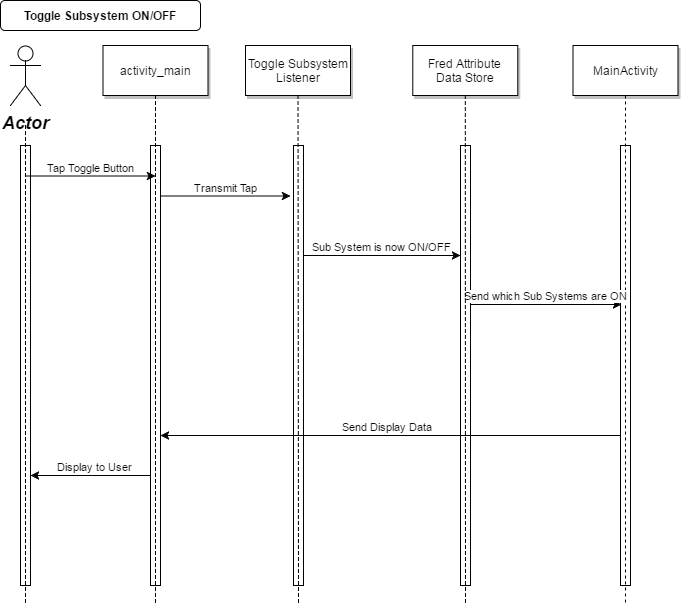
\includegraphics[width=0.7\linewidth]{../Resources/Toggle_Subsystem_Sequence_Diagram.png}
	\caption{Sequence Diagram for Toggling Subsystem ON/OFF}
\end{figure}

\begin{figure}[H]
	\centering
	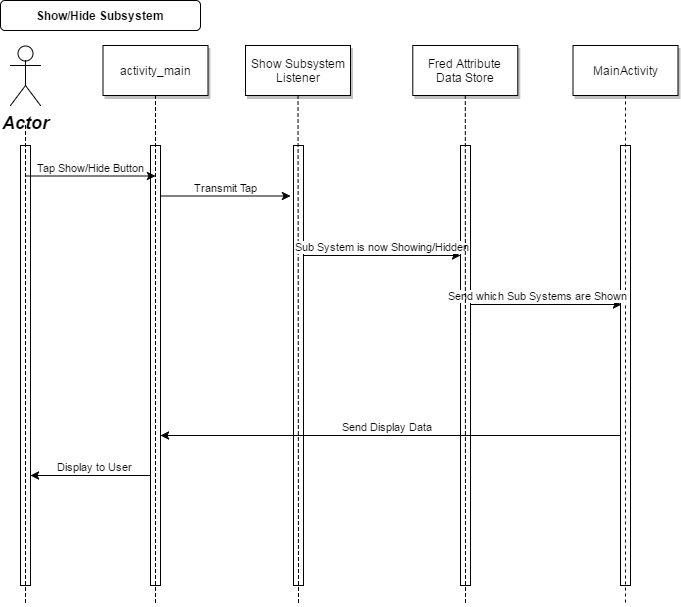
\includegraphics[width=0.7\linewidth]{../Resources/Show_Subsystem_Sequence_Diagram.png}
	\caption{Sequence Diagram for Showing/Hiding Subsystem}
\end{figure}
\begin{figure}[H]
	\centering
	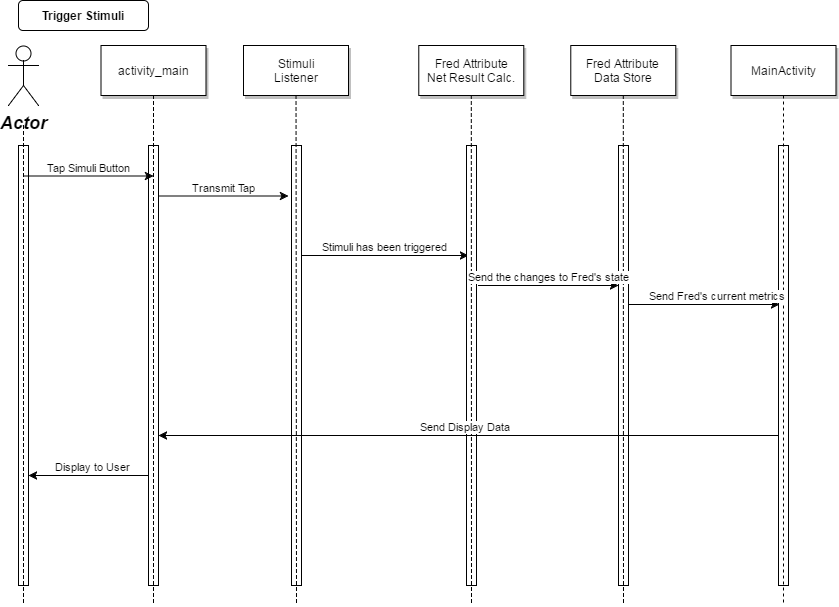
\includegraphics[width=0.7\linewidth]{../Resources/Trigger_Stimuli_Sequence_Diagram.png}
	\caption{Sequence Diagram for Triggering Stimuli}
\end{figure}
% End Section

\section{Detailed Class Diagram}
\label{sec:detailed_class_diagram}
% Begin Section
Given below is the detailed class diagram for the selected architecture. The diagram is divided into five packages which span the various main modules of the application.
Some of the classes differ from the activity class diagram given in the overall architecture design document (deliverable 2) due to the fact that later exploration of the chosen
architecture led to new insights on a more reasonable way to implement the software project.

\begin{figure}[H]
	\includegraphics[width=1.0\linewidth]{../Resources/ClassDiagram.png}
	\caption{Detailed Class Diagram}
\end{figure}
% End Section

\newpage

\appendix
\section{Division of Labour}
\label{sec:division_of_labour}
% Begin Section
\begin{tabular}{l c r}
	\textbf{Name} & \textbf{Work Completed} & \textbf{Signature} \\
	
	Kunal Shah &  & 
	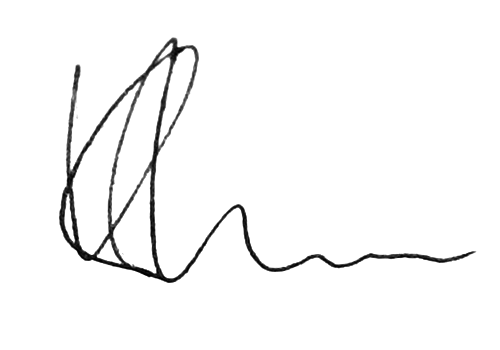
\includegraphics[scale=0.2]{../Resources/Signature/Kunal-Sig.png} \\
	
	Gabriel Castagner &  &
	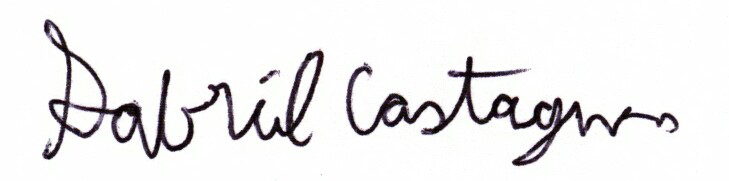
\includegraphics[scale=0.2]{../Resources/Signature/Gabe-Sig.png} \\
	
	Victor Velechovsky &  & 
	
\includegraphics[scale=0.3]{../Resources/Signature/Vic-Sig.png} \\
	
	Josh Mitchell & Sequence Diagrams & 
	
\includegraphics[scale=0.2]{../Resources/Signature/Josh-Sig.png} \\
\end{tabular}
% End Section

\end{document}
%------------------------------------------------------------------------------